%%%%%%%%%%%%%%%%%%%%%%%%%%%%%%%%%%%%%%%%%%%%%%%%%%%%%%%%%%%%%%%%%%%%%%%%%%%%%
%%%
%%% File: utthesis2.doc, version 2.0jab, February 2002
%%%
%%% Based on: utthesis.doc, version 2.0, January 1995
%%% =============================================
%%% Copyright (c) 1995 by Dinesh Das.  All rights reserved.
%%% This file is free and can be modified or distributed as long as
%%% you meet the following conditions:
%%%
%%% (1) This copyright notice is kept intact on all modified copies.
%%% (2) If you modify this file, you MUST NOT use the original file name.
%%%
%%% This file contains a template that can be used with the package
%%% utthesis.sty and LaTeX2e to produce a thesis that meets the requirements
%%% of the Graduate School of The University of Texas at Austin.
%%%
%%% All of the commands defined by utthesis.sty have default values (see
%%% the file utthesis.sty for these values).  Thus, theoretically, you
%%% don't need to define values for any of them; you can run this file
%%% through LaTeX2e and produce an acceptable thesis, without any text.
%%% However, you probably want to set at least some of the macros (like
%%% \thesisauthor).  In that case, replace "..." with appropriate values,
%%% and uncomment the line (by removing the leading %'s).
%%%
%%%%%%%%%%%%%%%%%%%%%%%%%%%%%%%%%%%%%%%%%%%%%%%%%%%%%%%%%%%%%%%%%%%%%%%%%%%%%

%%%%%%%%%%%%%%%%%%%%%%%%%%%%%%%%%%%%%%%%%%%%%%%%%%%%%%%%%%%%%%%%%%%%%%%%%%%%%
%%%
%%
%% This file, and the corresponding tcdthesis.sty the accompanied it, have
%% been modified for the M.Sc. styles used in Trinity College, Dublin
%%
%%
%%%%%%%%%%%%%%%%%%%%%%%%%%%%%%%%%%%%%%%%%%%%%%%%%%%%%%%%%%%%%%%%%%%%%%%%%%%%%
\documentclass[a4paper, 12pt, oneside]{report}         %% LaTeX2e document.
\usepackage{algorithm,algorithmic}
\usepackage {tcdthesis}              %% Preamble.
\usepackage{hyperref}
\usepackage{graphicx}
\usepackage{float}
\usepackage[T1]{fontenc}
\usepackage{array}

\mastersthesis                     %% Uncomment one of these; if you don't
% \phdthesis                         %% use either, the default is \phdthesis.

\thesisdraft                       %% Uncomment this if you want a draft
                                     %% version; this will print a timestamp
                                     %% on each page of your thesis.

\leftchapter                       %% Uncomment one of these if you want
%\centerchapter                      %% left-justified, centered or
% \rightchapter                      %% right-justified chapter headings.
                                     %% Chapter headings includes the
                                     %% Contents, Acknowledgments, Lists
                                     %% of Tables and Figures and the Vita.
                                     %% The default is \centerchapter.

% \singlespace                       %% Uncomment one of these if you want
\oneandhalfspace                   %% single-spacing, space-and-a-half
% \doublespace                       %% or double-spacing; the default is
                                     %% \oneandhalfspace, which is the
                                     %% minimum spacing accepted by the
                                     %% Graduate School.

\renewcommand{\thesisauthor}{Salil Ajgaonkar}            %% Your official TCD name.
\renewcommand{\thesismonth}{August}                  %% Your month of graduation.
\renewcommand{\thesisyear}{2018}                      %% Your year of graduation.
\renewcommand{\thesistitle}{Proof Of Concept for Opportunistic Security in MPLS Networks}            %% The title of your thesis; use mixed-case.
\renewcommand{\thesisauthorpreviousdegrees}{ B.E}  %% Your previous degrees, abbreviated; separate multiple degrees by commas.
\renewcommand{\thesissupervisor}{Stephen Farrell}      %% Your thesis supervisor; use mixed-case and don't use any titles or degrees.
% \renewcommand{\thesiscosupervisor}{}                %% Your PhD. thesis co-supervisor; if any.

% \renewcommand{\thesiscommitteemembera}{}
% \renewcommand{\thesiscommitteememberb}{}
% \renewcommand{\thesiscommitteememberc}{}
% \renewcommand{\thesiscommitteememberd}{}
% \renewcommand{\thesiscommitteemembere}{}
% \renewcommand{\thesiscommitteememberf}{}
% \renewcommand{\thesiscommitteememberg}{}
% \renewcommand{\thesiscommitteememberh}{}
% \renewcommand{\thesiscommitteememberi}{}


\renewcommand{\thesisauthoraddress}{25, Liffey Walk, North Lotts, Dublin 1}

\renewcommand{\thesisdedication}{XXXX}     %% Your dedication, if you have one; use "\\" for linebreaks.


%%%%%%%%%%%%%%%%%%%%%%%%%%%%%%%%%%%%%%%%%%%%%%%%%%%%%%%%%%%%%%%%%%%%%%%%%%%%%
%%%
%%% The following commands are all optional, but useful if your requirements
%%% are different from the default values in tcdthesis.sty.  To use them,
%%% simply uncomment (remove the leading %) the line(s).

\renewcommand{\thesisdegree}{Master of Science in Computer Science}  
                                     %% default is "DOCTOR OF PHILOSOPHY"
                                     %% for \phdthesis or "MASTER OF ARTS"
                                     %% for \mastersthesis.  Provide the
                                     %% correct FULL OFFICIAL name of
                                     %% the degree.
\renewcommand{\thesisdegreestream}{(Future Network Systems)}
                                     %% Default is empty. This is used on
                                     %% the title page of the thesis.

\renewcommand{\thesisdegreeabbreviation}{M.Sc.}
                                     %% Use this if you also use the above
                                     %% command; provide the OFFICIAL
                                     %% abbreviation of your thesis degree.
\renewcommand{\thesistype}{Dissertation}    %% Use this ONLY if your thesis type
                                     %% is NOT "Thesis" for \phdthesis
                                     %% or \mastersthesis.
                                     %% Provide the OFFICIAL type of the
                                     %% thesis; use mixed-case.

% \renewcommand{\thesistypist}{...}  %% Use this to specify the name of
                                     %% the thesis typist if it is anything
                                     %% other than "the author".

%%%
%%%%%%%%%%%%%%%%%%%%%%%%%%%%%%%%%%%%%%%%%%%%%%%%%%%%%%%%%%%%%%%%%%%%%%%%%%%%%



\begin{document}                                  %% BEGIN THE DOCUMENT

\thesistitlepage                                  %% Generate the title page.

\thesisdeclarationpage                %% Generate the declaration page.

\thesispermissionpage                 %% Generate the copyright permission page

%\thesisdedicationpage                             %% Generate the dedication page.

\begin{thesisacknowledgments}                     %% Use this to write your
First and foremost I would like to thank my thesis advisor Dr. Stephen Farrell of the School of Computer Science and Statistics at Trinity College Dublin whose guidance and expertise has given me wealth of knowledge which I shall forever carry with me.

I would also like to acknowledge Dr. Donal E. O'Mahony of the School of Computer Science and Statistics at Trinity College Dublin as the second reader of this thesis, and I am gratefully indebted to his very valuable comments on this thesis.

Finally, I would like to express my extreme gratitude to my parents without whose support I would have never been able to be the man I am today. Who constantly encouraged and pushed me to be the best I can be and have been a source of unfailing support and encouragement throughout my years of study. This accomplishment would not have been possible without them. Thank you.

%% acknowledgments; it can be anything
\end{thesisacknowledgments}                       %% allowed in LaTeX2e par-mode.

\begin{thesisabstract}                          %% the abstract for your thesis

Multiprotocol Label Switching (MPLS) is a high performance packet switching technology which supports packet switching for multiple protocols and access technologies. It is a switching technology that redirects data based on short label paths rather than an IP table lookup. Each Label Switched Router in the MPLS network has a table that tells the router how to handle and redirect specific types of data. This helps the router to handle data in a consistent fashion while maintaining flexibility for traffic engineering at the same time.

MPLS provides networking corporations and government high speed and reliable data transfer over geographically dispersed sites while maintaining flexibility and high bandwidth data exchange. It is very easy to scale and can be efficiently tuned to meet various service level requirements. it is primarily used to provide Virtual Private Network (VPN) services for corporations who wish to transfer private data over a public network.

Such a heavy reliance on MPLS by big companies and the general public to manage their data means that any forms of network attacks often have the potential to disrupt vital everyday operations. Attacks ranging from data theft to denial of service if successful may lead to severe damages to the service provider as well as the owner of the data.

Earlier work conducted by the Internet Engineering Task Force (IETF) have analyzed the various vulnerabilities and security threats that affect the MPLS technology and have drafted a potential resolution to some of the security issues. This work proposed the implementation of Opportunistic Security in the MPLS network using payload encryption to encrypt the underlying application data and protocols headers using symmetric key encryption between end to end or hop by hop Label Switching Routers (LSRs) on an MPLS Label Switched Path (LSP).

This thesis describes the proof of concept for this proposed solution by implementing it on an experimental controlled environment and measuring its effects on the overall functionality and features of the presently running MPLS technology, the results of which should give an idea regarding the feasibility of the solution in practical commercial network in the world.  
\end{thesisabstract}

\begin{thesissummary}                           %% The summary page for your thesis

MPLS is a network routing technology which uses circuit switching and packet switched network technologies to support data routing for multiple protocols. It is a protocol independent and highly scalable technology whose flexibility enables efficient utilization of network resources resulting in high quality of service at low cost. MPLS relies on the use of fixed bytes of data that represent as labels for routing decisions. These labels are pushed on top of a data packet at the ingress (entering) switch of an MPLS network. All the succeeding Label Switching Routers (LSRs) in the MPLS cloud lookup these labels to appropriately route the data to the correct destination. The path to the destination is pre-configured in the LSR's label lookup table rather than an IP routing table. This avoids any complex lookups or reading long network addresses and implementation of longest match algorithms. Once the MPLS packet reaches the egress (exiting) switch of the MPLS network, the MPLS label is popped off and the data packet is then transmitted as a regular original packet along the succeeding switches. The LSRs between the ingress and the egress switch of the MPLS cloud also have the capability of pushing and popping off the MPLS labels on the data packet to efficiently engineer the network traffic.

	Networking corporations and service providers leverage this flexibility to scale their network services. Using the advantages of MPLS they are able to run high bandwidth applications over seamless IP based networks that connect multiple, remote site \cite{grayson2009analysis}. The reliance on MPLS VPNs by corporations and government agencies means that attacks ranging from intercepting sensitive data to disrupting data, voice and multimedia services can significantly impact vital operations \cite{mpls-os-internet-draft}.

	Previously in MPLS, data security in the MPLS network mainly relied on just three features: \\
    1) Physical isolation of MPLS networks that ensured interception of MPLS traffic was not possible. \\
    2) Higher-layer protocol security such as IPsec which had been used whenever a particular flow has determined that security was desirable \cite{grayson2009analysis}.\\
    3) Layer 2 protocol security like MACSec where security was implemented on a hop by hop basis between devices connected on the Ethernet. 
    However these features have a number of vulnerabilities. The network is still vulnerable to network taps between links, misconfiguration of routers, data replication, at the same time users might not enable to implement end to end security in their applications \cite{grayson2009analysis}.
    
    To mitigate these vulnerabilities to some extent, the IETF drafted an Internet-draft titled "Opportunistic Security in MPLS Networks draft-ietf-mpls-opportunistic-encrypt-03" which proposed a novel idea of implementing Opportunistic Security (OS) in the currently existing MPLS implementations. The Internet draft suggested the implementation of opportunistic encryption of data payload which is held by the MPLS packet using symmetric key encryption. As the LSR's only rely on the information contained in the MPLS labels for routing, the contents of the MPLS packet are of no significance for the flow of traffic. Thus end-to-end or hop-by-hop encryption of the data payload of the MPLS packet by the LSRs may contribute to maintaining the confidentiality, integrity and authenticity of the data that flows through the MPLS network.
    
    This dissertation describes a way to implement this proposed experimental idea in a controlled environment by simulating the flow of traffic in an MPLS network in a virtual network and comparing the difference in performance between MPLS with the OS and MPLS without the OS. This will help validate or invalidate the proposed solution experimentally and further spread more light on its impact and feasibility on real world implementation.
    
    This experiment is carried out using an experimental network setup consisting of mininet as a virtualized network platform. On this virtual platform OpenVSwitch (OVS) virtual switches are setup which simulate the flow of network traffic through the virtual switches. The MPLS flows needed to configure the OVS switches are configured using OpenFlow Software Defined Networking (SDN) Technology. OpenFlow configures these OVS switches by installing flow rules to simulate the behavior of an MPLS switch. The Opportunistic Security feature in the MPLS is implemented by coding the symmetric key functionality into the existing OVS code base which would then be configured onto the OVS switches in the mininet network to simulate the behavior of the system with the OS. We then evaluated the performance of the system by measuring certain network performance metrics and compared them with the ones measured without the OS. This comparative analysis may help us understand the performance level of the OS in MPLS against MPLS without OS, if there are any room for improvements and its potential impact on practical implementation. 
 \end{thesissummary}


\tableofcontents                                  %% Generate table of contents.
\listoftables                                     %% Uncomment this to generate list of tables.
\listoffigures                                    %% Uncomment this to generate list of figures.

%%
%% Include thesis chapters here...
%%
  \chapter{State Of The Art}
MPLS  by itself is vulnerable to a number of security threats. This is primarily because MPLS in its primary idea aims to solve the problem of high speed data delivery over large geographical network while maintaining flexibility so it can be scaled to meet business requirements. Routing and traffic engineering using MPLS is very easy and service providers can leverage this benefit to provide varying levels of Quality of Service.

With the increasing deployment of MPLS, security of data passing through the MPLS network has become a grave concern for corporations and the service provider alike. Service providers are concerned with the security and confidentiality of their customers data while corporations using MPLS to share data between their geographically distributed sites demand authentication and integrity as well.

\section{Security Requirements in MPLS}
Some of the General Service Provider Security Requirements are as follows:

\subsection*{Protection of data at the Data-Plane}
Encryption of data is not provided as a basic feature in all telecommunication protocols. Protocols like IPSEC have all the features of authentication, data integrity and confidentiality however it is not widely adopted by all applications. however, roughly 30\% of web sites actually take on this burden of implementing IPSEC, even though the software required is ubiquitous [2].

\subsection*{Protection from attacks on Label Distribution protocol}
In [16] the authors have stated that attacks on Label Distribution protocol (LDP) exploit 3 weaknesses: The LDP specification, Service provider implementation and underlying infrastructure. The authors have expressed that these attacks can lead to various DOS attacks or Route modification attacks most of which ma lead to violation of SLA for the Service provider. Naturally the Service provider would like protection against such attacks as a major requirement in implementing MPLS networks.

\subsection*{Prevent Malicious External Controllers from misconfiguring the SDN switches}
SDN Switches are vulnerable to being misconfigured by external controller. An attacker can send malicious control-plane messages to the switches which can misconfigure them to send packets to a malicious switch, replicate the packets or drop the packets in general to trigger a Denial of service attack (DOS). Service providers expect some form of authentication of messages received from the control plane by the switches to make sure any control-plane messages received by the SDN are from a legitimate controller in the network.

\subsection*{Prevention of attacks that spoof IP addresses}
Many attacks on protocols running in a core involve spoofing a source IP address of a node in the core (e.g., TCP-RST attacks).[3] If such a spoofed IP address gets accepted in the MPLS network, the MPLS switches can route sensitive packets to the spoofed address leading to data leakage. The attacker can then have the luxury to analyses and read the data at his leisure till the systems identifies the spoofed address.

\subsection*{Hiding Service Infrastructure}
In general the service provider would like to hide his service infrastructure from the external network. An MPLS/GMPLS provider may make its infrastructure routers unreachable from outside users and unauthorized internal users. For example, separate address space may be used for the infrastructure loopbacks [3]. A service that is hidden to the external network has less chances of being targeted by attackers.

\subsection*{Protection from mis-merging of LSP}
Care needs to be taken that any implementation of security procedures do not alter the the MPLS Label stacking logic which then becomes vulnerable to mis-merging of LSPs. LSP mis-merging has security implications beyond that of simply being a network defect. LSP mis-merging can happen due to a number of potential sources of failure, some of which are due to MPLS label stacking [17].

\subsection*{Link Authentication}
Service providers would prefer to authenticate a site before linking a connection. this helps validate the site based on certain security protocols like IPSEC. If the user wishes to hold the authentication credentials for access, then provider solutions require the flexibility for either direct
authentication by the PE itself or interaction with a customer authentication server [3].

\subsection*{Security Considerations in Operations, Administration, and Maintenance messages}
Operations, Administration, and Maintenance (OAM) messages are messages that are used for the internal functionality of the MPLS switches. OAM messages help in monitoring devices and implementing data transport mechanisms on a network level. They are responsible for the overall performance of the network device. On a service-oriented functionality they provide monitoring services to end users which is vital to keep a track of the performance so as to make sure the SLAs are met.The nature of OAM therefore suggests having some form of authentication, authorization, and encryption in place. This will prevent unauthorized access to MPLS-TP equipment and it will prevent third parties from learning about sensitive information about the transport network [18]

Meeting these requirements can easily fail if the system in place is vulnerable to any security threatening attacks. With the intention of securing these vulnerabilities we first need to analyze what are the different forms of attacks and how we can resolve them. A number of research has been conducted in analyzing the various security threats that plague the MPLS networks.

\section{Security threats in MPLS}
 \cite{GRAYSON2009146} has analysis a number of security threats to MPLS in VPN. In this work the authors have discussed the principal security issues in MPLS related to Network separation, Inter-provider connectivity and MPLS packet labeling. In [2] the authors have stated that security in MPLS previously relied only on the physical isolation of the MPLS network and High-layer protocol security like IPSec. The authors have also gone further as to why these features fall short of being the ideal solutions to current network attacks.In [3] the authors have elaborated on specific types of exploits that threaten the MPLS/GMPLS network. The authors have segregated the attacks in the form of attacks on the data plane, attacks on the control plane, attacks on the operation and management plane and insider attacks. they have also recommended defensive techniques for MPLS against these forms of attacks. In \cite{Alouneh2009} the author has suggested a mechanism to enhance the security in MPLS networks by using multi-path routing using a threshold secret sharing scheme. In [8] has elaborated the security issues that are inherent in the MPLS architecture. The authors state that some routers may implement security procedures relying on certain headers being in fixed place relative to a certain layer header in the IP stack. Another security issue mentioned was that the MPLS routers agree on the meaning of the labels and thus work upon a chain of trust to transfer data in the network and that if packets from untrusted sources are accepted then they may get routed illegitimately.
 
In this section we will try to list out the various security attacks that the MPLS network is vulnerable to. The Security attacks have been categorised into 4 types: Attacks on the Data Plane, Attacks on the Control Plane, Attacks on Operational and Management of the MPLS Network and Insider attacks.
    
\subsection{Attacks on the Data Plane}
Attacks that are mainly aimed at the User's or the Service Provider's data are categoried into Data-plane security attacks. These attacks aim to either manipulate the data flowing through the MPLS network, delete the data flowing through the MPLS network, inject malicious data or just plain observe data unauthorized data all with malicious intent.

\subsubsection{Plain IP forwarding}
MPLS Switches can forward un-labelled IP packets as normal IP packets if they are configured to do so. An attacker already inside the core can exploit this information to reach other core devices compromising them. It is difficult to manage this type of attack by just traffic engineering or implementing any VPN service.

\subsubsection{Forwarding captured packets from the core to the outside network}
An attacker inside the core can capture the data sensitive packets and forward them to any destination he desires even if IP traffic is not being forwarded. This can be done by encapsulating the captured packet in the payload of a UDP packet. The source IP address can be spoofed and the detination  IP address can be set to whever the attacker may wish to forward the packet. This however is only possible if the attacker is already aware of the Labels needed to route through the LSP.

\subsubsection{Sniffing of Data}
Data sniffing can be explained as the action of capturing data packets and analyzing its contents to understand what they contain. Private corporations and Users in general often transfer confidential and sensitive data over the internet. If this data is not sufficiently encrypted before forwarding them onto the internet then an attacker can use the wide variety of packet sniffing tools to sniff these data sensitive packets and use the sensitive information in them for malicious purposes. Unauthorized packet sniffing can also be a first step in other attacks in which the recorded data is modified and re-inserted, or simply replayed later [3]. Unauthorized packet sniffing is one of the most commonly faced security issue in any network system including and especially the MPLS network considering its wide spread use for mission critical systems and reliance of both common users as well as Multi national corporations.

\subsubsection{Modification of Data Packets}
If an attacker is able to manipulate the contents of the data passing through the MPLS network then he has the potential to initiate a wide range of security attacks on the network. Though not as easy as it sounds the attacker must first be aware of the internal configurations of the MPLS netowork which more often than not is more difficult than the actual manipulation of packets. MPLS often has an "egg-shell" security model where it is very difficult to penetrate the internal network core, but once inside the attacker can cause a lot of damage to the service provider and the network service as a whole [1]. Some of the potential attacks that can be triggered by data manipulations are:

\subsubsection{Route modification attacks}
Once inside the network an attacker can manipulate the data flowing through the network and route them to any destination he desires, provided he has the information necessary to route the information correctly through the network. Route modification attacks enable an attacker to gain access to certain traffic (e.g., maneuver traffic through a compromised link); affect accounting (e.g., trigger automatic financial transactions among cooperating providers); or route traffic across domains (e.g., send one customer’s traffic to another customer’s network) [16].

\begin{enumerate}
\item Path Switching:
A normal traffic flowing through the MPLS network ideally follows a fixed set path or to be more precise an Label Switched Path (LSP). The LSP is determined by the initial traffic engineering setup done by the service provider. The traffic engineering primarily relies on the label configuration of the packets. If an attacker were to modify this label information of a data packet, then he may be able to route the data packet that it was not intended to. Such a path is called a rogue path. By doing this the attacker can deceive the traffic engineering and reap benefits out of it. For example
an attacker can forward his online gaming data packets via the live video conferencing path to get better speed advantage and disrupting the video conferencing quality of service.

\item Destination Switching:
Just like Path switching, an attacker is also able to modify the destination of a packet if he modifies the label configurations appropriately. This can fool the MPLs network into forwarding the packet to a rogue destination where the attacker can further conduct malicious operations on the packet which he wasn't able to do while inside the MPLS network.

\item Brute-Force Label Prediction:
An attacker can deduce the LSP of an MPLS network if the destination address is known. He can target this address and pass data packets into the MPLS
with an initial label value. He can then test out the Label with incremental values till he receives a reply from the destination address. The reply from the destination address can help him deduce the LSP for the destination address and thus reuse the label information to further pass data to the destination. 

\item Brute Force Target Location:
Similar to label prediction, the target can also try to identify what type of service lies at the end of an LSP, for example if the user were trying to identify if a web service lies at the end of an LSP then he can set the target tcp port to 80 and incrementally try out the IP address for a successful hit. This however is a very time consuming process considering the probabilities of getting the correct IP address compared to the total combination of IP addresses possible.

\item Forward Equivalency Class (FEC) Specificity Exploitation:
When configuring the MPLS network Packets are configured in such a way that packets of similar type are routed through the same LSP. These packets are thus bound by the same MPLS label and routed through the same path as designated for labels of that value. Such classification of packets is termed as Forward Equivalency Class. This attack takes advantage of the “most specific” or “longest match” rule applied by ingress routers to incoming IP
packets. An attacker needs access to a link or a connection to an interface to establish an LDP session. The attacker identifies a target FEC and
advertises label bindings for more specific FECs. LSRs that receive the label mappings distribute them throughout the network, thereby building
new LSPs toward the compromised link [16].

\item Label Mapping Messages Modification:
An attacker can modify the Label values of a datapacket inside the MPLs network. He can thus reroute the traffic or create loops within the MPLS network. This modified message is sent on to the next MPLS switch. When the upstream LSR receives a packet for the target FEC, it applies the incorrect
label, which causes the downstream router to mistakenly recognize the packet as belonging to a different FEC. The packet is then forwarded
along the desired LSP [16].

\item Address Messages Modification:
Similar to label modification an attacker can redirect a data packet by spoofing the the destination IP address. This attack, also known as Fabricating Address Messages, reroutes traffic or creates loops by manipulating the “least cost” mechanism used to select the next hop. Traffic can be redirected using access to a compromised link adjacent to an LSR along a selected LSP. This modified message forces the LSR to adjust its local label information base and generate a Label Request message.Thus, a new LSP is constructed that forces the targeted traffic along the compromised link [16].

\item Label Edge Router (LER) label Modification:
Label Edge Router (LER) are routers situated at the end of an MPLS network. These routers are the final routers in the MPLS network that pop the final MPLS Label off the data packet and forward the data packet its original form before entering the MPLS network. This attack requires access to a link
along the path between VPN sites. Redirection of packets to a different site in the same VPN requires the attacker to know the routes and labels corresponding to that site. The attack is executed by modifying the topmost label of a transit packet (before the penultimate pop) to another label. If the new label is valid at the next hop, the packet is forwarded to a different LER [1]. This new LER may or may not be connected to the destination. It could either drop the packet as a whole which could lead to denial of service if the attacker modified to many of the packets or the LER may forward the IP packet as a normal IP packet, depending on its configuration.

\item VPN label Modification:
VPN label modification is similar to the LER Label Modification. In this type of attack two VPNs are involved. One is the legitimate source VPN and the other is the destination VPN which is incorrect. The attacker captures and modifies the datapacket label of the source VPN and redirects it to the incorrect VPN. When this modified data packet reaches the LER, the LER redirects it to the incorrect VPN. If the LER doenot have a VRPN routin gand Forwarding (VRF) Table then the LER may forward the packet as a regular IP packet. Given knowledge of routes and VPN labels in the network core, the combination of VPN label modification with LER label modification (previous attack) enables an attacker to redirect and/or drop any traffic passing through the compromised link [1].

\item VRF table Modification:
A more serious issue is if the attacker is able to modify the VRF tables themselves. This would grant the user the ability to control the traffic from the LER. The attacker can change outgoing LER labels and outgoing VPN labels to impact QoS. More over, the attacker can control the routes taken by ingress VPN traffic and divert it to the wrong VPNs [1].
\end{enumerate}

\subsubsection{Data Insertion attacks}
    	Insertion of Inauthentic Data Traffic: Spoofing and Replay
    	Injection Based on VPN Labels:
    	Injection Based on LER Labels:
        
    Unauthorized Deletion of Data Traffic
    Unauthorized Traffic Pattern Analysis
               
    Misconnection
    
    Denial-of-Service Attacks
    	Modifying the Community Attribute in LERs:
    	Fabricating Notification Messages:
    	Blocking KeepAlive Messages:
    	Fabricating Address Withdraw Messages
    	Fabricating Label Withdraw Messages:
    	Exhausting Label Memory:
    	Creating Loops:
    	LSP Deletion.
    	Path State Resource Exhaustion.
    	Excessive LSP ID Allocation.

\subsection{Attacks on the Control Plane}
	LSP Creation by an Unauthorized Element
    LSP Message Interception
    Attacks against RSVP-TE
    Attacks against LDP
    Denial-of-Service Attacks on the Network Infrastructure
    Attacks on the SP’s MPLS/GMPLS Equipment via Management Interfaces
    Cross-Connection of Traffic between Users
    Attacks against Routing Protocols
    
\subsection{operation and managemnet}
	MAlicious collaborator
   	Unauthorizd access to LER
    misconfiguration 6

\subsection{insider attacks}

19)
\subsection{Enumeration attacks}
	Ingress Probing
    Record Route Object Access.
\subsection{Cross domain attacks}
	Promiscuous Path Acceptance.
    Pre­Labeled Traffic Acceptance.

refer the book number 5 for ending paragraph

Most of the literature covering MPLS security usually concerned itself with a certain use case. \cite{GRAYSON2009146} [11][12][15] analyzed the security issues of MPLS VPN. [3] concerned with the security framework to be implemented for the MPLS network. [8] elaborated on the security concerns in implementing label stack encoding. We therefore need to summarize a set of security threats that is commonly faced by MPLS network as well as the existing security tools to identify the pros and cons of implementing them and determine if the implementation of the OS in MPLS is justifiable or not.

\section{Exisiting security tools}
Several Security tools already exists to make MPLS more secure. Each tool having its own set of features and complexities to make data transmission over MPLS network more secure. A thorough analysis needs to be made regarding which tool to be used based on the operational requirements and feasibility of its implementation in the current scenario. There is no one single tool that solves all the security issues plaguing the MPLS network, however proper consideration and analysis of the security requirements of the system and using the appropriate tool to mitigate them is more than enough to make MPLS secure enough for business requirements. Based on this idea it is best to have a suitably large number of security tools in the arsenal to fight off the possible security threats. Security tools range from a wide variety of mechanism to make MPLS secure. some of which are described in the following.

\subsection{Payload Encryption}
One of the ways to make MPLS more secure is to encrypt the data that is to be passed through it. This prevents any sniffing attacks from sniffing any confidential data that a company or service provider may be transmitting via the MPLS network. Packet Encryption is ideally a responsibility of the application that is sending or receiving the data. Applications can use security tools like Transport Layer Security (TLS) which is an Internet standard to implement privacy and data integrity between communicating computer applications.

IPsec is another tool which can be applied end-to-end or hop-by-hop applications to maintain privacy and data integrity. It is mainly used to encrypt IP packets that flow through the network. IPSec can be used to encrypt the IP packets before they are passed onto the MPLS network. IPsec has historically placed a heavy "full-mesh" configuration burden on implementation although this is now ease with the introduction of the NULL Authentication Method in the Internet Key Exchange Protocol Version 2 allows for opportunistic key exchange to support IPsec [1].

\subsection{Link layer security}
Moving down the IP stack, encryption is also possible in the Layer 2 (Link Layer). Packets can be encrypted on a hop by hop basis between two communicating routers using MACsec. MACsec encrypts Ethernet frames that transmit across ethernet network. Thus end to end security can be implemented by creating a chain of trust between all the participating routers in the network path.

\subsection{Pseudowires}
MPLS is used to transport data of multiple protocols like Ethernet, ATM, TDM along with IP. Security tools limited by protocol types often don't help in fully leveraging the strengths of MPLS networks. Security tools that work for all types of protocols go well with MPLS implementation. Such a tool is pseudowire (PW) encryption. PW security is carried out by setting up pseudowires that tunnel the native service through the MPLS core by encapsulating at the edges [13]. The benefits of PW encryption is that compromising of edges or routers becomes very difficult. Protection of control plane messages means protection from majority of attacks.PEs are usually configured to reject MPLS packets from outside the
service provider network, thus ruling out insertion of PW packets \cite{GRAYSON2009146}
from the outside [13]


The reason why MPLS does not provide encryption or any other data confidentiality features is because in a conventional IP networks, every router in a network ideally analyses IP packet headers to process it. Encryption will add additional overhead and delay in the network [10x]. However with the increasing implementation of MPLS in mission critical applications the added data integrity, confidentiality and authentication may outweigh the overhead introduced. To get a better judgment of the cost to benefit ratio this project aims to calculate the overhead cost involved in implementing this opportunistic security in MPLS networks which can further strengthen or weaken the case of its feasibility in real life implementation.




1) payload encryption 1
2) Link layer security 1
3) Encryption on Pseudowires 1
4) Management System Authentication 13
5) p2p authentication 13
6) IPSEC in MPLS 13
7) Diffserv 13
8) Encryption for Device Configuration and Management 13
9) Access Control Techniques, Filtering, 
	\section{Section 1.1}

  \chapter{Design}
\section{Description}
\section{Mininet}
\section{OpenVSwitch (OVS)}
\section{Network Setup}
\section{OS changes in OVS}

mininet
OVS
mininet + ovs = h1,h2,h3,s1,s2,s3
mpls setup
changes in ovs (CW, encryption GCMAES, DECRYPTION)

  \chapter{Experiment}
In the previous chapter we described the design details that we will be using to implement the experiment. In this Chapter we go into the implementation details of the project.

\section{Infrastructure setup}
We will start of by first setting up the virtual network with the OVS Switches running the traditional MPLS System. To do this we first set up the mininet virtual network with the OpenVSwitch switches and hosts as described in Figure 2.5. Once the network system is in place we add the MPLS flows to the switches using OpenFlow. And finally we run a ping test to pass the ICMP packets through the MPLS switches to test the system.

\subsection{Setting up Mininet and OpenVSwitch}
The Mininet tool package is available in the Advanced Package Tool (APT) of all Linux Distributions. It can be easily installed on the system using the package name 'mn'. The Mininet package has a dependency on OVS packages and thus are installed along with the mininet package by the APT command.\\
\\
The Network topology can be set up by calling the command:\\
\\
\textit{sudo mn --topo=linear,3 --switch=ovsk --controller=ovsc}\\
\\
The parameter meanings are as follows:
\begin{enumerate}
\item --topo=linear,3 \\
This parameter creates a topology of 3 switches each with their own host connected in a linear fashion.
\item --switch=ovsk \\
This parameter determines the type of switch that will be created in the mininet network. The value 'ovsk' indicates that OVS switches that run in kernel space are to be created
\item --controller=ovsc \\
This parameter determines the type of controller that will be created in the mininet network. this controller is responsible for forwarding the flow rules and actions to all the switches in the network. the value 'ovsc' indicates that an OVS controller is to be created to communicate with the OVS switches.
\end{enumerate}


\section{Testing the MPLS System}
\subsection{Addition of the MPLS flows}
Once the network infrastructure is set up we then add the MPLS Flows to the switches via the OVS controller. This is done passing the flow rules and actions to the Openflow Switch Manager (ovs-ofctl).\\
\\
The OpenFlow Switch management command structure is as follows: \\
\\
\textit{ovs-ofctl -O OpenFlow13 add-flow s1 "table=0,in\_port=1,eth\_type=0x800,actions=goto\_table:1}"
\\
\begin{enumerate}
\item -O OpenFlow13\\
Indicates the OpenFlow Version to use. The value 'OpenFlow13' indicates OpenFlow Version 1.3.
\item add-flow s1\\
Indicates the action to be taken on the switches. We can add flows, delete flows modify flows etc using the OpenFlow Protocol. The value 's1' indicates the switch on which the flow rules are to be added.
\item "table=0,in\_port=1,eth\_type=0x800,actions=goto\_table:1" \\
Is the flow rule where the flow is to be added in table '0' of the Switch, to packets arriving at port '1' which is mapped to interface s1-eth1, which are of eth type 0x800 (ICMP Packets). The 'actions' value indicates the type of actions to take on such packets.
\end{enumerate}

The Complete Flow configuration for MPLS is as follows:

\begin{figure}[H]
       \centering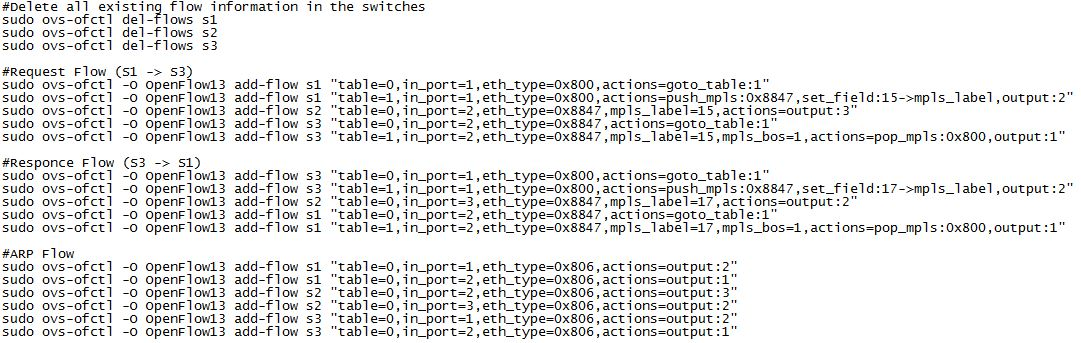
\includegraphics[width=\textwidth]{images/10_Open_Flow_flows_for_MPLS.JPG}
       \caption{OpenFlow Flow Scripts for traditional MPLS}
       \label{fig:compbest}
\end{figure}

\subsection{Testing Communication for MPLS}
After adding the Flow Rules we can initiate the ping test from h1 to h3 by calling the ping command in the Mininet CLI. This would create an ICMP packet at Host H1 which would be forwarded to Switch S1. Switch S1 based on the Flow Rules as described in Figure 3.1 will forward the packet to its table '1' where it will push an MPLS label of eth value 0x8847, set its label value to 15 and forward it to switch S2. Switch S2 will redirect all packets of eth type 0x8847 and MPLS Label value 15 to Switch S3. S3 based on its flow rules will first forward the data packet to its table 1 where it will check if the MPLS label has value 15 and is a bottom of the stack label, pop the MPLS label if it is and later forward the packet to Host H3. H3 then responds to the ICMP request by sending the ICMP response to switch S3 after which the data packets is subjected to the flow rules as described in the 'Response Flow' part of the diagram.

To test if the packets are being routed correctly using MPLS labels we can inspect the packets at switch 2. This is done by calling the command 'tcpdump' on one of the interfaces of switch 2. Refer diagram

\begin{figure}[H]
       \centering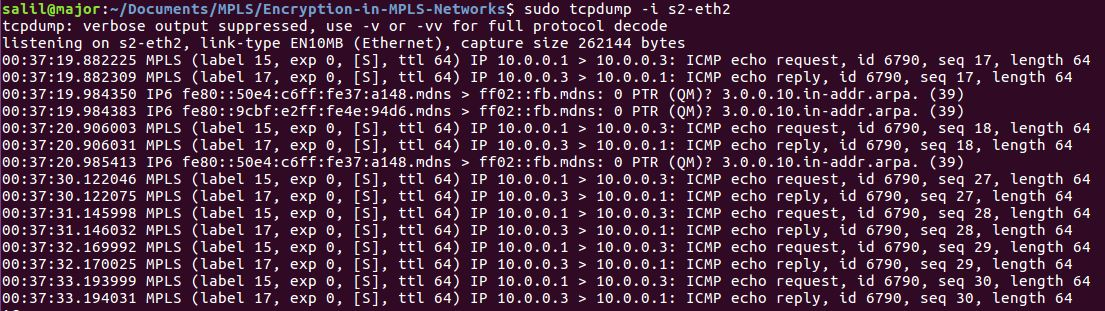
\includegraphics[width=\textwidth]{images/11_TCP_Dump_Capture_for_MPLS.JPG}
       \caption{'tcpdump' response for MPLS network traffic}
       \label{fig:compbest}
\end{figure}

The output displayed by the ping command in diagram indicates that the switches are pushing, inspecting and popping the MPLS labels correctly without any issues as shown in Figure 3.3.

\begin{figure}[H]
       \centering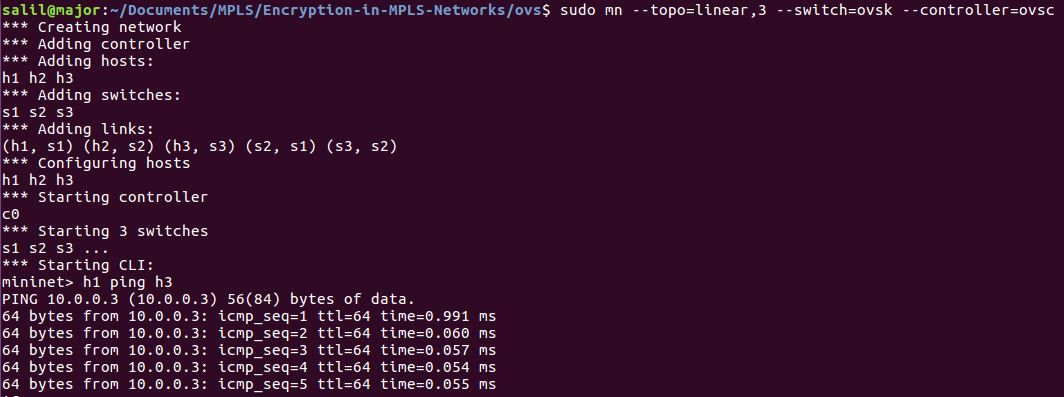
\includegraphics[width=\textwidth]{images/12_ICMP_responce_for_MPLS.JPG}
       \caption{'ping' response for MPLS Network Traffic}
       \label{fig:compbest}
\end{figure}


\section{Implementation of OS Encryption functionality}
The next part of the experiment involves the implementation of the OS Encryption functionality. Based on the OS designed as mentioned in chapter 2, the four additional functionality involved in the MPLS OS is the addition and removal of the CW and the Encryption and Decryption of the MPLS Payload. These functionalities should be performed by the OVS Switch involved in the network experiment and as such should be implemented in the OVS code base. 

After a thorough study of the OpenVSwitch codebase, we found out that there is no such inbuilt provision in the OVS codebase for the required Os functionality. We can neither implement the CW functionality nor the Encryption/Decryption of the MPLS payload with the currently existing features of OVS. The functionality was thus needed to be implemented manually into the OVS codebase and then converted into a kernel module for the Switches to implement the same at the kernel level.

For the sake of development classification we will segregate the OS functionality into 2 categories:

\subsection{Changes at the Ingress (Entering) Switch}
When the ICMP request packet from H1 enters S1, before pushing the MPLS header on the data packet, S1 first encrypts the payload data using AES-GCM encryption algorithm. The key and IV required for the encryption is currently hardcoded in the code as their values are dependent on the Key Exchange which is not implemented in this project. The AEAD-AES-GCM encryption is carried out using the Linux Kernel Crypto API\footnote{Kernel Crypto API is a cryptographic framework in the Linux Kernel for various kernel implementations dealing with cryptography}. After encryption the pseudo wire CW is pushed on top of the encrypted data followed by pushing the MEL on top of it.

Due to certain implementation aspects of the Linux Kernel Crypto AEAD encryption API, instead of encrypting the Payload data first and then adding the CW we will first add the CW and then encrypt the underlying Payload. The details of this aspect will be discussed further in this section.

\subsubsection{Insertion of CW}
We first create the CW data structure in the OVS codebase and assign the nonce value to the CW sequence attribute. 

%insert CW structure

In OVS datapath and Linux kernel in general, all data packets are parsed into a fundamental data structure called a socket buffer (skb)\footnote{The socket buffer, or "SKB", is the most fundamental data structure in the Linux networking code. Every packet sent or received is handled using this data structure.}. The skb is a series of contiguous memory location storing the data packet information in the form of bytes. The structure of the skb is shown in Figure 3.4.

\begin{figure}[H]
       \centering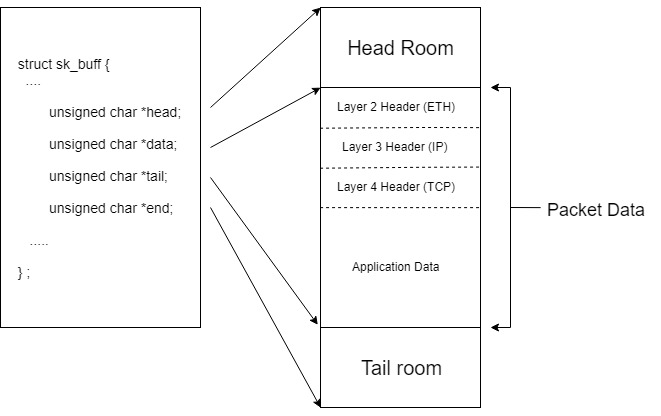
\includegraphics[width=\textwidth]{images/13_SKB_Data_Structure.jpg}
       \caption{SKB Data Structure}
       \label{fig:compbest}
\end{figure}

Any changes that involve manipulating the data packet have to be done by manipulating the data bits of the skb data structure. A number of data pointers help map the various data and header locations in the skb structure. The linux kernel has in-built APIs to manipulate these contents. It is highly recommended to use these API's as the various pointer in the skb data structure are heavily interdependent on each other. Using these APIs we manipulate the data packet and insert our CW between the payload and the MAC header of the datapacket. This is done by calling the following series of Kernel APIs. Refer Table 3.1 which depicts the implementation of the skb kernel APIs to insert the CW into the data packet.\\

\begin{table}[H]
\centering
\begin{tabular} { | m {0.9cm} | m {5cm} | m {8cm} | }
\hline
Sr.no & Command & Function \\
\hline
\hline
 1 & skb\_cow\_head & Checks if space, the size of the CW header, is available in the headroom for inserting the CW. \\ 
 \hline
 2 & skb\_push & Allocates the space for the Data Structure. \\ 
 \hline
 3 & memmove & Moves the MAC header to the newly allocated space so that the CW can be inserted between the MAC header and the underlying payload. \\
 \hline
 4 & skb\_reset\_mac\_header & Resets the MAC header pointer to the new MAC header position.  \\
 \hline
 5 & skb\_mac\_header(skb) + skb->mac\_len & Points to the start of the CW memory space where the CW data bits can be filled. \\
\hline
\end{tabular}
\caption{Steps to insert CW in Data packet}
\label{table:1}
\end{table}

\subsubsection{Encryption of Data using Linux Crypto API}
The Linux Kernel Crypto API is a rich set of cryptographic ciphers and data transformation API used for cryptographic operations at the kernel level. To understand and properly use the Crypto API functions one needs to understand their underlying architecture specifications and the functional flow of these APIs.

The Kernel Crypto API refers to all encryption algorithms as 'transformations'. The encryption is carried out by 2 major components, The transformation object, also called 'Cipher Handles' and the request handle. The transformation object contains all the settings and configurations of the given encryption type to use. The request handler as the name suggest handles the encryption request.

\begin{table}[H]
\centering
\begin{tabular} { | m {0.9cm} | m {5cm} | m {8cm} | }
\hline
Sr.no & Command & Function \\
\hline
\hline
 1 & Initialize 'crypto\_aead' and 'aead\_request' & Initialize the AEAD transformation Object and its Request Handler \\ 
 \hline
 2 & crypto\_alloc\_aead & Allocate the AEAD Cipher Handle\\ 
 \hline
 3 & aead\_request\_alloc & Allocate the AEAD Request Handle \\
 \hline
 4 & aead\_request\_set\_callback & Set the Asynchronous callback function that will be executed once the encryption is successfully completed \\
 \hline
 5 & crypto\_aead\_setkey & Set the encryption key in the cipher handle \\
  \hline
 6 & aead\_request\_set\_crypt & Set the data buffers where the encryption process will happen. The data that is to be encrypted is concatenated with the allocated data at the start and then passed as whole as plain text \\
 \hline
 7 & aead\_request\_set\_ad & Set the associated data information that will be used to generate the authentication tag for authentication of data at the receiving end \\
 \hline
 8 & crypto\_aead\_encrypt & Start the encryption process\\
\hline
\end{tabular}
\caption{Steps to Encrypt the Data Payload}
\label{table:1}
\end{table}

Table 3.2 describes the flow of API calls to initiate the encryption of the packet data.

Once the payload data has been encrypted S1 can then further push the MEL label on top of the packet followed by the Special Purpose Label Packet and another normal MPLS packet for routing.

\subsection{Changes at the Egress (Exiting) Switch}
Once the encrypted MPLS OS packet reaches the Egress Switch S3, S3 pops the top MPLS label along with the MEL. It then inspects nonce value in the CW header. If the nonce counter value matches with the counter value of switch S3 then the switch moves ahead with the decryption. 

\subsubsection{Decryption of Data using Linux Crypto API}
Decryption of the MPLS payload follows the same procedure as the one during Encryption process with a slight change in the input values to the API's. During decryption, the cipher text is passed in the place of plain text into the API's. The cipher text is a concatenated combination of the associated data, ciphertext and authentication tag. Also in the crypto\_aead\_encrypt function the flag is set to decrypt. The decryption process authenticates the packet using the authentication tag. The process can send out an alert if the authentication tag fails to authenticate. The output of the decryption gives us a concatenated combination of the associated data and the plain text. 

\subsubsection{Removal of CW}
Just as how we used the in-built SKB manipulation APIs to insert the CW in the Ingress Switch, we will use the same approach while removing the CW from the Data packet. Refer Table 3.3 which depicts the implementation of the skb kernel APIs to remove the CW from the data packet.

\begin{table}[H]
\centering
\begin{tabular} { | m {0.9cm} | m {5cm} | m {8cm} | }
\hline
Sr.no & Command & Function \\
\hline
\hline
 1 & skb\_postpull\_rcsum & Recalculate the checksum after pulling the MEL from the data packet\\ 
 \hline
 2 & memmove & Moves the MAC header to occupy the place where the CW resides \\ 
 \hline
 3 & \_\_skb\_pull & Pulls the CW size equivalent of data from the top of the data structure which was redundant as the MAC header shifted down.  \\
 \hline
 4 & skb\_reset\_mac\_header & Resets the MAC header pointer to the new MAC header position.  \\
 \hline
 5 & skb\_set\_network\_header & Sets the network header pointer to the new network header position. \\
\hline
\end{tabular}
\caption{Steps to remove the CW from the Data packet}
\label{table:1}
\end{table}


\section{Testing the MPLS OS System}
Once the OS functionality has been implemented in the OVS code-base we need to deploy it into out experimental system for testing. This is done by first building the code base to create its binaries. The OVS code has a Make files that has all the file building sequences scripted into it. Using the Linux 'make' command you can compile the system. Once the System has compiled successfully you call the Linux function 'make install' to install all the binaries into the appropriate locations in the system. We then remove the currently loaded OVS module by calling 'rmmod openvswitch' function so we can load the new module containing the MPLS OS functionality. We then run the 'make modules\_ install' function to build the kernel module libraries and install them the the Kernel modules directory. Finally we load the newly installed openvswitch kernel module by calling 'modprobe openvswitch'.

\subsection{Addition of the MPLS OS flows}
The MPLS Flows for OS are similar to the ones mentioned for traditional MPLS. The only difference being the addition of the Special Purpose Label with value 15, the MEL and the CW. However the addition of these headers is not a part of the OpenFlow Flow. The addition of these headers depends on the success of Key Exchange between the Ingress and Egress LSR's before the OS can begin and thus the LSRs must be programmed to take that decision programmatically. Since we are not implementing the Key exchange in this experiment and have hard coded the key for experimental purposes. We are allowed to instruct the LSRs to force push the MEL of value 1 followed by the Special purpose MPLS Label with value 15 and another MPLS Label for routing purposes. Addition of CW is programmed internally in the OS functionality.
	During Experimentation however, it was observed that the Egress switch would drop these packets. The MPLS OS packets would route through switch S2 but S3 would drop these packets before forwarding to Host H3. Analysis into the issue led to the discovery of issues in OVS with respect to contiguous popping off of 2 or more Labels (MPLS and even VLAN). It was observed that at the kernel level OVS is only able to push and pop one Label. 2 or more contiguous labeled packets are routed to the Userspace for efficient handling. However for some reason the Userspace fails to do so. This issue is apparently prevalent in OVS and concerns were been raised back in 2016. However no information was found regarding its solution. More details can be found in this mailing list \cite{OVSmail1} \cite{OVSMail2}
    As a result a work-around was implemented which would not affect the overall aim of the project. Instead of pushing the MEL, the special purpose MPLS label with value 15 and the normal MPLS Label, we decided to push just one MPLS Label of label value 1. This Label will act as a functional combination of all the 3 labels in our experiment and would not interfere with the OS Encryption as a whole.
    So based on this work-around the Flow configuration for MPLS with OS is as follows:
    
\begin{figure}[H]
   \centering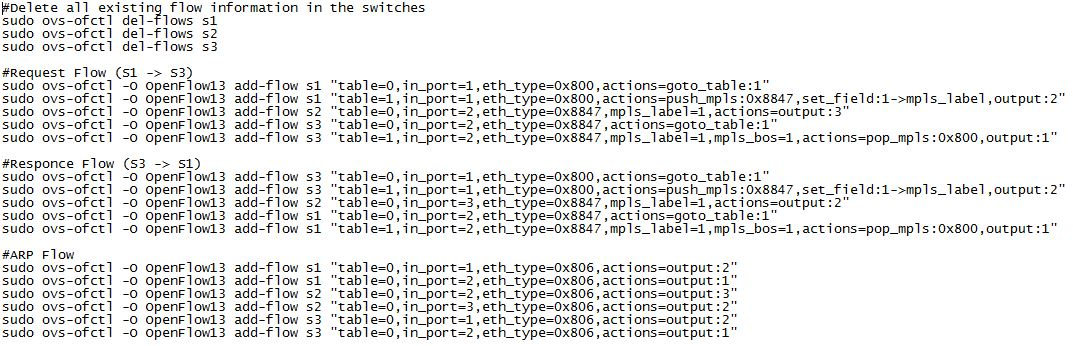
\includegraphics[width=\textwidth]{images/14_Open_Flow_flows_for_MPLS_OS.JPG}
   \caption{OpenFlow Flow Scripts for MPLS with OS}
    \label{fig:compbest}
\end{figure}

\subsection{Testing Communication for MPLS with OS}
The behavior of the MPLS System with the OS is similar to the behavior without the OS. The only difference to note is that in the MPLS OS Switch S1 will be encrypting the data packet and inserting the CW along with the MPLS Label with value 1 before forwarding it to Switch S2. S2 must not be able to sniff the internal data of the encrypted packet and must be able to forward it only based on the MPLS Label value. Once the MPLS OS packet reaches Switch S3, S3 should decrypt the packet, remove the CW and pop the MPLS Label before forwarding the original ICMP packet to host H3. Host H3 will respond to the packet with the response ICMP packet which follows the reverse path with encryption on S3 and decryption on S1.

To test if the packets are being encrypted correctly using the MPLS OS, we can inspect the packets at one of S2's interface. This is done by calling the command 'tcpdump' on one of the interfaces of switch 2. Refer diagram

\begin{figure}[H]
   \centering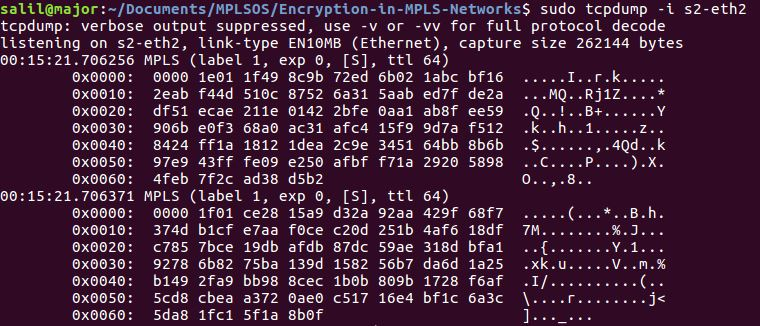
\includegraphics[width=\textwidth]{images/15_TCP_Dump_Capture_for_OS.JPG}
   \caption{'tcpdump' response for MPLS OS}
    \label{fig:compbest}
\end{figure}

As we can see in Figure 3.6 tcpdump tries to sniff the contents of the data packets and is unable to interpret its contents. The only understandable part being the MPLS header with value 1. The rest of the contents is dumped as it is in hexadecimal byte form. S2 cannot interpret that the contents of the IP packet are infact ICMP as we saw during the communication testing of traditional MPLS system in section 3.2.2.

The output displayed by the ping command in Figure 3.7 displays the proper response being received for each ICMP request packet. This means that the receiving switch is able to correctly decrypt the packet at its end and get the original ICMP packet as was sent by the sender.

\begin{figure}[H]
   \centering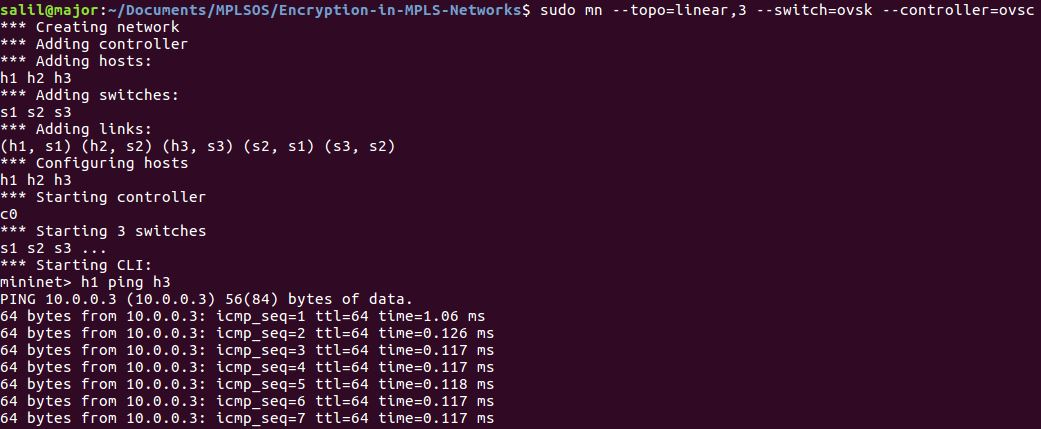
\includegraphics[width=\textwidth]{images/16_ICMP_responce_for_MPLS_OS.JPG}
   \caption{'ping' response for MPLS OS}
    \label{fig:compbest}
\end{figure}












  \chapter{Results}
\section{Analysis of the metrics}
\section{Results}
  \chapter{Future Work}
  \chapter{Conclusion}


% \begin{thebibliography}{ieee}                   %% Start your bibliography here; you can
% \bibliography{refs}                               %% also use the \bibliography command
% \end{thebibliography}                             %% to generate your bibliography.

\bibliographystyle{ieee}
\bibliography{refs}



\addcontentsline {toc}{chapter}{Appendices}       %% Force Appendices to appear in contents
\begin{appendix}
The Codebase of this entire experiment and results found are uploaded on a github repository with the link:\\
 \textbf{https://github.com/SalilAj/Encryption-in-MPLS-Networks}
% \include{appendix2}
\end{appendix}


%\addcontentsline {toc}{chapter}{Bibliography}     %% Force Bibliography to appear in contents


\end{document}                                    %% END THE DOCUMENT
